
%(BEGIN_QUESTION)
% Copyright 2011, Tony R. Kuphaldt, released under the Creative Commons Attribution License (v 1.0)
% This means you may do almost anything with this work of mine, so long as you give me proper credit

Sketch the necessary tube connections to build a working pneumatic flow-control loop.  Note the three shut-off valves, each one intended to provide a source of instrument air to each of the three field instruments:

$$\includegraphics[width=15.5cm]{i00886x01.eps}$$

Also, determine if this controller needs to be {\it direct-acting} or {\it reverse-acting} in order to make the loop work.

\underbar{file i00886}
%(END_QUESTION)





%(BEGIN_ANSWER)

Award 8 points for proper diagram, 2 points for correct action:

$$\includegraphics[width=15.5cm]{i00886x02.eps}$$

The controller needs to be {\bf reverse-acting}.

%(END_ANSWER)





%(BEGIN_NOTES)

{\bf This question is intended for exams only and not worksheets!}.

%(END_NOTES)


